\documentclass[preprint,11pt]{elsarticle}

\usepackage{fontspec}
\usepackage{amsmath,amssymb}
\usepackage{graphicx}
\usepackage{booktabs}
\usepackage{tabularx}
\usepackage{array}
\usepackage{multirow}
\usepackage{siunitx}
\usepackage{lineno}
\usepackage[hidelinks]{hyperref}
\usepackage{xcolor}
\usepackage{caption}
\captionsetup{font=small,labelfont=bf}
\graphicspath{{figures/}}
\sisetup{detect-all}
\newcommand{\pp}{\,pp}
\newcommand{\Rr}{\ensuremath{\mathrm{R}\!\to\!\mathrm{T}}}

\journal{Journal of Neuroscience Methods}

\begin{document}

\begin{frontmatter}

\title{Shared presentation order leaks through subject-independent evaluation of fNIRS decoders: identifiability, a validated two-step diagnostic, and a multi-dataset audit}

\author[aff1]{Pinzhen He\corref{cor1}}
\cortext[cor1]{Corresponding author.}
\ead{baijihuixun@163.com}
\address[aff1]{Independent Researcher, Tokyo, Japan}

\begin{abstract}
\textbf{Background:} Leave-one-subject-out (LOSO) evaluation is regarded as protection against temporal confounds in brain decoding. When every participant receives the same condition sequence, session position, carry-over and drift align with the labels in held-out subjects too.

\textbf{New method:} A two-step diagnostic. Step 1 decodes the upcoming condition from a window ending before the block and any cue (null-window probe); step 2 trains on those windows and tests on task windows (rest-to-task transfer). We add design-only ceilings, identifiability analysis, source-separating conditional decoding and permutation statistics, validated by simulation.

\textbf{Results:} Eight public EEG/fNIRS datasets share one order. Latin squares rotated across subjects balance position but not transitions: the previous condition alone predicted the current one with 80\% accuracy. In simulation, the probe was at chance under noise and conditional decoding attributed sources correctly; step 1 did not predict task-decoding inflation, step 2 did. In real fNIRS, null windows carried order information in Shin 2018 ($n=26$) and Tufts fNIRS2MW ($n=68$) for six decoders. In Shin it arose from previous-block carry-over and did not reach task windows (transfer $\le 0$); in Tufts' final blocks 42--100\% of task-decoding accuracy was obtainable from pre-cue windows. A per-subject-order control was at chance.

\textbf{Comparison with existing methods:} Prior work treated subject-independent splits as the remedy for temporal confounds; we show when that fails, how to detect it and when it matters.

\textbf{Conclusions:} Order should be randomised per participant; LOSO studies on shared-order data should report both diagnostic steps.
\end{abstract}

\begin{highlights}
\item Eight public EEG/fNIRS datasets present one condition order to all participants.
\item Latin squares across subjects balance block position but not block transitions.
\item A null-window probe detects order information under leave-one-subject-out.
\item Rest-to-task transfer predicts when that information inflates task decoding.
\item Validated with ground-truth simulation, six decoders and a negative control.
\end{highlights}

\begin{keyword}
fNIRS \sep EEG \sep mental workload \sep data leakage \sep cross-validation \sep experimental design \sep carry-over
\end{keyword}

\end{frontmatter}
\linenumbers

%% ============================================================================
\section{Introduction}
\label{sec:intro}

Decoding mental workload from functional near-infrared spectroscopy (fNIRS), alone or with EEG, relies increasingly on public benchmarks \citep{shin2018,huang2021,chen2023}. Reported accuracies on the same data range from above 90\% (within-subject) to 39--56\% for three classes under subject-independent evaluation \citep{benerradi2023,khan2026}. Subject-independent evaluation, typically leave-one-subject-out (LOSO), is the standard prescription against leakage \citep{brookshire2024}.

Temporal confounds in block designs are well documented within subjects: classifiers can decode recording time instead of the stimulus \citep{li2021,ahmed2022,xu2026}, filtering moves information backwards across onsets \citep{vandriel2021}, and pre-stimulus decoding serves as a sanity check \citep{grootswagers2017}. When these analyses were repeated across subjects, accuracy fell to chance \citep{li2021,ahmed2022,xu2026}, and subject-independent splitting came to be seen as a remedy.

That remedy assumes that a held-out subject's temporal structure is unrelated to the labels learned from the others. It fails when every participant receives the same condition sequence: block position, the preceding condition, rest durations and slow drift are then aligned with the label in the same way for everyone. An fMRI study noted this possibility in passing \citep{barbu2015}. Whether it affects EEG/fNIRS benchmarks, how large it is, which of the aliased sources produces it, and whether it changes reported task-decoding accuracy have not been established.

We address these questions with a design-level and a data-level analysis (Table~\ref{tab:novelty}). At the design level we compute how much label information a sequence carries by itself and when its temporal sources are identifiable. At the data level we propose a two-step diagnostic, validate it in simulation with known ground truth, apply it to three public fNIRS datasets and six decoders, and re-run three published methods.

\begin{table}[htbp]
\centering
\caption{Relation to prior work on temporal confounds in neural decoding.}
\label{tab:novelty}
\footnotesize
\begin{tabularx}{\textwidth}{@{}>{\raggedright\arraybackslash}p{3.3cm}>{\raggedright\arraybackslash}X>{\raggedright\arraybackslash}p{4.2cm}@{}}
\toprule
Work & What it shows & What is added here \\
\midrule
Li 2021; Ahmed 2022 \citep{li2021,ahmed2022} & Block-design EEG decodes time within subjects; LOSO restores chance & Conditions under which LOSO does \emph{not} restore chance \\
Xu 2026 \citep{xu2026} & Autocorrelation leaks with no neural signal (within subject) & Cross-subject case; sources identified \\
van Driel 2021 \citep{vandriel2021} & Zero-phase filters create pre-onset decoding & Causal/no-filter controls; filter phase inflates by $\sim$7\pp \\
Grootswagers 2017 \citep{grootswagers2017} & Pre-stimulus decoding as a sanity check & Pre-cue windows under LOSO, plus rest-to-task transfer \\
G\"orgen 2018 \citep{gorgen2018} & Decode design variables to expose confounds (fMRI) & Design-only ceilings; transitions vs position \\
Barbu 2015 \citep{barbu2015} & Shared order may confound cross-subject fMRI decoding (remark) & Quantified in three datasets, six decoders \\
Kilgallen 2025; Hu 2021 \citep{kilgallen2025,hu2021} & Repeated / shared stimuli inflate accuracy & Shared \emph{order}, not stimulus identity \\
\bottomrule
\end{tabularx}
\end{table}

%% ============================================================================
\section{Materials and methods}
\label{sec:methods}

\subsection{Census of presentation order}
We examined public EEG and fNIRS datasets used for decoding and distributed with continuous recordings or event timing. Order was read from released event files (BrainVision markers, NIRx event files, BIDS \texttt{events.tsv}, MATLAB marker structures) where possible; documentation-only cases are marked.

\subsection{Datasets analysed}
\textbf{Shin et al.\ 2018 n-back} \citep{shin2018}: 26 participants, fNIRS (36 channels, \SI{10.4}{Hz}) and EEG (28 channels); 0-, 2- and 3-back blocks of \SI{40}{s} preceded by a \SI{2}{s} instruction and followed by \SI{20}{s} rest; three runs of nine blocks. The three run orders differ but are identical across participants. Word generation (WG) from the same session, with per-participant random trial order, served as negative control.
\textbf{Tufts fNIRS2MW} \citep{huang2021}: 68 participants, frequency-domain fNIRS (\SI{5.2}{Hz}); 16 n-back blocks (0--3-back, $\sim$\SI{83}{s}). Probes used the raw release; benchmark analyses used the official filtered task segments and 30\,s windows.
\textbf{Chen et al.\ 2023 Stroop} \citep{chen2023}: 21 participants, fNIRS (20 channels, \SI{100}{Hz}); four \SI{32}{s} blocks (neutral or incongruent).
\textbf{PhysioNet mental-fnirs} \citep{mukli2021}: 12 participants; four $\sim$\SI{134}{s} blocks in the fixed order 0-, 1-, 0-, 2-back.

\subsection{Two-step diagnostic}
\label{sec:diagnostic}
\emph{Step 1, null-window probe.} For each block we take a window that ends before the block and before any cue about it (Shin: ending \SI{2}{s} before the instruction; Tufts: ending at the instruction, inside the rest after the previous block) and decode the upcoming condition with LOSO. Above-chance accuracy shows that the design and the signal together carry order information that a held-out subject shares.

\emph{Step 2, rest-to-task transfer (\Rr).} A decoder trained only on null windows is tested on task windows (20--24\,s or 20--30\,s after onset) of the held-out subject. Above-chance transfer shows that the order information is present in the task window in the same form, so it can contribute to task-decoding accuracy. The ratio \Rr/task gives the share of task accuracy obtainable without task data.

\emph{Preprocessing controls.} (a) Filtering: zero-phase, causal (minimum-phase) band-pass, causal low-pass only, or none. (b) Offset removal: a label-free per-recording constant (recording mean, or a strictly causal mean over data before all probe windows); no per-block baselines. (c) Windows never overlap cue periods.

\emph{Features and classifier.} Per-channel window mean and least-squares slope; standardisation and L2 logistic regression ($C=0.1$); per-subject balanced accuracy, so chance is $1/k$ whatever the class counts.

\emph{Statistics.} Per-subject LOSO accuracies are not independent because folds share training data \citep{varoquaux2018}. Our primary test is a permutation test \citep{ojala2010} in which, within each subject, the assignment of labels to blocks is permuted and the entire LOSO pipeline is re-run (500 permutations); this preserves fold dependence, class counts and the pairing of null and task windows from the same block, and corresponds to a per-subject random order. In simulation (Section~\ref{sec:res-sim}) this test was close to nominal but not exact, so only $p<0.01$ is treated as primary evidence. For deep networks, where permutation was too costly, we report one-sided Wilcoxon tests and bootstrap intervals with the same threshold.

\subsection{Design-only ceilings and identifiability}
For a given assignment of orders to subjects we compute the Bayes-optimal accuracy of predicting a block's condition from its position alone, or from the previous condition alone, pooled over subjects and with no signal. To assess identifiability we regress the null-window level on block position, previous load and previous rest duration with subject fixed effects, and report the condition number of the design matrix.

\subsection{Conditional decoding}
\label{sec:conditional}
To separate carry-over from position and drift where the design permits it (Shin, whose three run orders differ), we decode the upcoming load from null windows separately within strata that hold one design variable fixed: blocks with the same previous load, or blocks at the same position within a run. Carry-over predicts that accuracy vanishes when the previous load is fixed and persists when position is fixed; drift predicts the opposite pattern for the previous-load stratum.

\subsection{Simulation}
\label{sec:sim-methods}
Synthetic HbO-like signals (8 channels, \SI{5}{Hz}, 40 subjects) comprised a load-dependent task response convolved with a double-gamma HRF (its tail is genuine carry-over), an optional extra post-block recovery term proportional to the previous load ($\kappa$), a slow drift whose group mean ($\mu$) is shared across subjects and whose individual deviation is not, an optional step per block position ($\phi$), subject offsets, cardiac/respiratory/Mayer oscillations and AR(1) noise. Timing followed Tufts (16 blocks) or Shin (three runs of nine). Designs: one shared order; shared order with load-dependent rest; Latin-square rows rotated across subjects; per-subject random order; per-subject random order under a common rule (no immediate repeats). Experiments: E1 calibration under pure noise (200 seeds per design); E2/E6 sensitivity and task-decoding inflation as functions of each component and of task effect size, with inflation defined as task accuracy with the component minus the same design and seed without it; E3 identifiability; E5 validation of conditional decoding with exactly one source switched on.

\subsection{Controls and reversed pairs}
\emph{Drift injection (Tufts).} Each participant's null-window vectors were shuffled across positions, then $k$ times the observed group-mean drift per position was added ($k\in\{0,0.25,0.5,1,2\}$, 20 repetitions).
\emph{Per-subject order (Shin WG).} Same participants, montage and pipeline as the n-back positive.
\emph{Reversed pairs (Chen).} Every participant saw neutral, incongruent, neutral, incongruent (recovered from the data; the descriptor states N-N-I-I). A condition decoder should be equally accurate on forward (neutral first) and reverse (incongruent first) pairs; a time decoder fails on the reverse pair.

\subsection{Benchmark of six decoders}
Logistic regression, RBF-SVM and random forest on mean/slope features; EEGNet, a reduced DeepConvNet and an LSTM on raw 10\,s windows (channels $\times$ 50 samples; fixed hyperparameters, no tuning on test subjects). ShallowConvNet was also run but did not decode the task itself reliably (task excess +1.5 to +3.7\pp, $p\ge0.019$), presumably because its squaring-and-log stage targets EEG band power, and it is not considered further. Each model was evaluated on step 1, step 2 and task decoding in Shin (no filter; causal) and Tufts (final blocks; 3-class and 0 vs 2).

\subsection{Re-running published methods}
\emph{BenchNIRS} \citep{benerradi2023}: package 1.7.1, published pipeline, with block markers shifted 12\,s earlier so that features lie before the instruction. \emph{Tufts DeepConvNet} \citep{huang2021}: official architecture, windows and 17 test buckets (CPU-limited grid). \emph{Con4m} \citep{chen2024con4m}: authors' code on one of 12 splits, with blocks re-concatenated in per-participant random order.

\subsection{Software and data availability}
Python (MNE, scikit-learn, PyTorch). Scripts \texttt{20\_}--\texttt{48\_} and \texttt{91\_}--\texttt{93\_} reproduce every number and figure from the public data: \url{https://github.com/huixun160/shared-order-audit}.

%% ============================================================================
\section{Results}
\label{sec:results}

\subsection{Shared order is common and sometimes misdescribed}
\label{sec:res-census}
At least eight public datasets present one sequence to every participant (Table~\ref{tab:census}, Fig.~\ref{fig:designs}). Shin and Tufts describe their orders as counterbalanced; both use a within-participant Latin square that is identical for all participants. In Tufts, rest after a block lasted 20, 20, 30 and 40\,s after 0-, 1-, 2- and 3-back (medians 20.0/20.0/29.6/39.8\,s), and every non-initial 0-back follows a 3-back. The Chen descriptor gives N-N-I-I; event codes and the authors' own per-condition files (17 of 19 checkable participants) show N-I-N-I. The Tufts raw release contains the first twelve blocks for only 9 of 68 participants; probes on Tufts therefore use blocks 14--16 (0-, 1-, 2-back), in which label and position are aliased.

\begin{table}[htbp]
\centering
\caption{Presentation order in public EEG/fNIRS datasets. ``Data'' = verified from released event files; ``Doc.'' = documentation only.}
\label{tab:census}
\footnotesize
\begin{tabularx}{\textwidth}{@{}>{\raggedright\arraybackslash}p{3.7cm}>{\raggedright\arraybackslash}p{1.8cm}r>{\raggedright\arraybackslash}X l@{}}
\toprule
Dataset & Modality & $N$ & Order & Source \\
\midrule
\multicolumn{5}{@{}l}{\emph{Shared by all participants}}\\
Shin 2018 n-back \citep{shin2018} & EEG+fNIRS & 26 & three 9-block run orders, identical for all & Data \\
Tufts fNIRS2MW \citep{huang2021} & fNIRS & 68 & 16 blocks \texttt{0123 1230 2301 3012}; rest length depends on load & Data \\
Tufts NIRS-X (audio n-back) & fNIRS & 53 & same 16-block sequence & Doc. \\
Chen 2023 Stroop \citep{chen2023} & EEG+fNIRS & 21 & N-I-N-I (descriptor: N-N-I-I) & Data \\
PhysioNet mental-fnirs \citep{mukli2021} & fNIRS & 12 & 0-1-0-2-back & Data \\
Ryb\'a\v{r} 2025 \citep{rybar2025} & EEG+fNIRS & 12 & identical stimulus sequence for participants 2--12 & Data \\
ZuCo 1.0/2.0 \citep{hollenstein2018} & EEG+eye & 12/18 & same sentences in same order & Doc. \\
High-altitude Stroop (Sci Data 2024) & EEG+fNIRS & 80 & one fixed 120-trial sequence & Doc. \\
\midrule
\multicolumn{5}{@{}l}{\emph{Randomised per participant}}\\
Shin 2018 word generation \citep{shin2018} & EEG+fNIRS & 26 & 24 distinct sequences; 10/10 per run & Data \\
COG-BCI \citep{hinss2023} & EEG & 29 & task order pseudorandomised per session & Data \\
\bottomrule
\end{tabularx}
\end{table}

\begin{figure}[htbp]
\centering
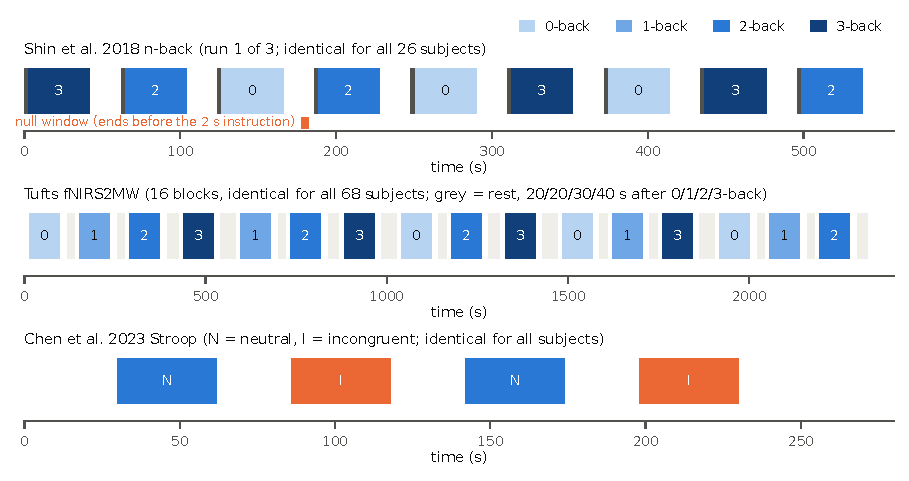
\includegraphics[width=\textwidth]{fig1_designs.pdf}
\caption{Block sequences shared by all participants in the three datasets analysed. Shin: grey bars mark the 2\,s instruction; the orange mark shows a null window. Tufts: grey segments are rest, whose length depends on the preceding load. Chen: the order recovered from the data.}
\label{fig:designs}
\end{figure}

\subsection{What the design alone allows, and what the diagnostic measures (simulation)}
\label{sec:res-sim}
\emph{Design-only ceilings} (Fig.~\ref{fig:sim}A). With the Tufts sequence, block position determines the condition (100\%) and the previous condition predicts it with 80\% accuracy (4 classes). Rotating Latin-square rows across subjects removes the position information (25\%) but leaves the transition information untouched (80\%), because every row is a cyclic shift of the same sequence. Per-subject random orders bring both to $\sim$28\%; a random order constrained by a rule common to all subjects (no immediate repeats) leaves 35\% from the previous condition. Balancing position across subjects therefore does not protect against carry-over; that requires sequences balanced for first-order residual effects \citep{williams1949} or per-subject randomisation.

\emph{Identifiability.} Over all 16 Tufts blocks, position and previous load are nearly uncorrelated ($r=-0.05$, condition number 1.06), and the regression recovered the true source in every simulated case (carry-over $\rightarrow$ previous load, $\beta=0.36$; drift $\rightarrow$ position, $\beta=1.11$; cross-terms $\le 0.02$). With load-dependent rest, previous load and rest duration were partly aliased (condition number 5.9), and in the final three blocks the design was singular (condition number $\sim 10^{16}$). Whether sources can be separated is thus a computable property of the design and of the blocks analysed.

\emph{Calibration.} Under pure noise the null-window probe was at chance in all designs (balanced accuracy 24.8--25.4\%). The within-subject permutation test rejected at $\alpha=0.05$ in 5.0\% (shared order), 7.5\% (Latin) and 9.0\% (random) of 200 runs; the Wilcoxon test behaved similarly (5.0, 7.0, 10.0\%). Both are close to nominal but not exact, which motivates the $p<0.01$ threshold.

\emph{Conditional decoding} (Fig.~\ref{fig:sim}B, Shin-like design). With carry-over only, null-window accuracy exceeded chance by 16.0\pp; holding the previous load fixed reduced this to 1.8\pp\ (the method's noise floor was 1.0--1.6\pp), while holding position fixed did not (27.5\pp). With drift only, the previous-load stratum retained 7.4\pp. A within-run position effect produced no leak, because Shin's run orders balance positions. The method thus distinguishes carry-over from drift.

\emph{Does step 1 predict inflation?} No (Fig.~\ref{fig:diag}A). Carry-over produced strong null-window information but no task-decoding inflation, because it decays before the task window. Drift and position effects persist into the task window, but inflated task accuracy only when the positions evaluated were unbalanced across classes (final three blocks: +1.4 to +6.0\pp); over all 16 blocks, where Tufts' Latin square equalises mean position across classes, they only added noise. Step 2 tracked inflation (Fig.~\ref{fig:diag}B; $r=0.65$, $p=5\times10^{-4}$ in the unbalanced case): transfer was negative for carry-over and positive for drift and position.

\begin{figure}[htbp]
\centering
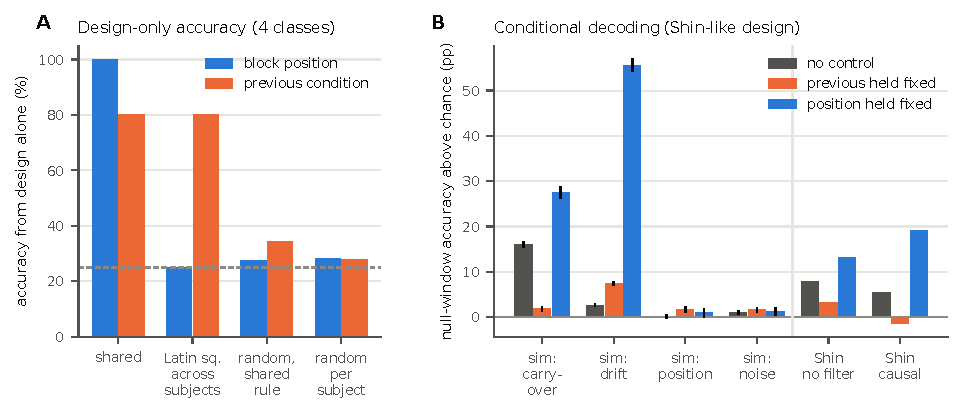
\includegraphics[width=\textwidth]{fig7_simulation.pdf}
\caption{Design-level analysis and validation. (A) Accuracy obtainable from the design alone (no signal), predicting the condition from block position or from the previous condition, for four ways of assigning orders to subjects. (B) Conditional decoding of null windows in simulated Shin-like data with exactly one source present (mean $\pm$ SEM over 10 seeds) and in the real Shin data.}
\label{fig:sim}
\end{figure}

\subsection{Step 1 in real data: order information before the cue}
In Shin, fNIRS null windows decoded the upcoming load above chance (Table~\ref{tab:probe}, Fig.~\ref{fig:null}A): causal band-pass 40.0\% ($p_{\text{perm}}=0.002$); unfiltered 38.3\% ($p_{\text{perm}}=0.012$, supporting). Zero-phase filtering inflated the effect by about 7\pp. EEG from the same windows was at chance. In Tufts' final blocks, null windows decoded the upcoming load at 48.0\% with recording-mean offset removal ($p_{\text{perm}}=0.002$) and at 39.2\% with a strictly causal baseline ($p_{\text{perm}}=0.048$, supporting). In the same participants, WG with per-subject order gave 51.8\% ($p_{\text{perm}}=0.14$). Across six decoders, null-window information was present in every model (Shin $+3.8$ to $+11.4$\pp; Tufts $+16.7$ to $+28.7$\pp; Table~\ref{tab:bench}).

\begin{figure}[htbp]
\centering
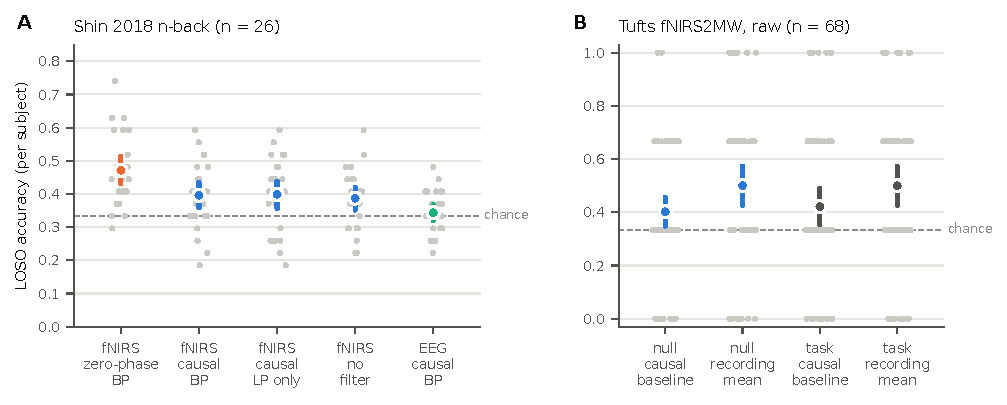
\includegraphics[width=\textwidth]{fig2_null_window.pdf}
\caption{Null-window probe, per participant (grey) with mean and bootstrap 95\% CI. (A) Shin n-back, fNIRS under four filters and EEG; windows end 2\,s before the instruction. BP, band-pass; LP, low-pass. (B) Tufts final blocks: null and task windows with a causal baseline or the recording mean.}
\label{fig:null}
\end{figure}

\begin{table}[htbp]
\centering
\caption{Two-step diagnostic in real data (logistic regression, permutation tests, 500 permutations; minimum attainable $p=0.002$). Excess over chance in percentage points.}
\label{tab:probe}
\footnotesize
\resizebox{\textwidth}{!}{%
\begin{tabular}{@{}llrrrrrr@{}}
\toprule
 & & \multicolumn{2}{c}{Step 1: null probe} & \multicolumn{2}{c}{Step 2: \Rr} & \multicolumn{2}{c}{Task decoding} \\
Dataset & Setting & excess & $p$ & excess & $p$ & excess & $p$ \\
\midrule
Shin n-back (3 classes) & causal band-pass & +6.7 & 0.002 & +5.6 & 0.002 & +14.0 & 0.002 \\
 & no filter & +5.0 & 0.012 & $-0.7$ & 0.69 & +12.0 & 0.002 \\
Tufts, blocks 14--16 (3 classes) & causal baseline & +5.9 & 0.048 & +4.0 & 0.004 & +5.5 & 0.004 \\
 & recording mean & +14.7 & 0.002 & +13.2 & 0.002 & +13.7 & 0.002 \\
Tufts, blocks 14--16 (0 vs 2) & causal baseline & +5.9 & 0.13 & +8.5 & 0.002 & +8.8 & 0.002 \\
 & recording mean & +20.6 & 0.002 & +20.4 & 0.002 & +20.3 & 0.002 \\
Shin WG (per-subject order) & causal & +1.8 & 0.14 & -- & -- & -- & -- \\
\bottomrule
\end{tabular}}
\end{table}

\subsection{Source of the leak in Shin: previous-block carry-over}
Shin's three run orders make carry-over and position separable. In the real data (Fig.~\ref{fig:sim}B), unconditional null-window accuracy exceeded chance by 7.9\pp\ (unfiltered) and 5.4\pp\ (causal); holding the previous load fixed reduced this to 3.3\pp\ ($p=0.08$) and $-1.4$\pp, whereas holding position fixed left 13.1\pp\ and 19.1\pp\ ($p\le 10^{-4}$). This matches the simulated carry-over signature and not the drift signature, which retains information when the previous load is fixed.

\subsection{Step 2: when order information enters task decoding}
In Shin without filtering, transfer was at or below chance for all six decoders ($-5.0$ to $-2.1$\pp; Fig.~\ref{fig:diag}C, Table~\ref{tab:bench}): the carry-over seen before the cue does not reach the task window, and Shin task accuracy is not explained by order. A causal high-pass changed this modestly (transfer 0--20\% of task accuracy), consistent with the filter carrying slow components forward in time. In Tufts' final blocks, 42--100\% of task-decoding accuracy (median 73\%, 3-class; 58--92\%, median 76\%, 0 vs 2) was obtainable from pre-cue windows alone, and with a strictly causal baseline transfer matched task decoding (0 vs 2: +8.5 vs +8.8\pp). Across all dataset--model combinations, transfer correlated with task accuracy ($r=0.73$, $p=5\times10^{-5}$). Within a dataset the conclusion was the same for every decoder; what differed was the dataset and preprocessing, as the simulation predicts.

\begin{figure}[htbp]
\centering
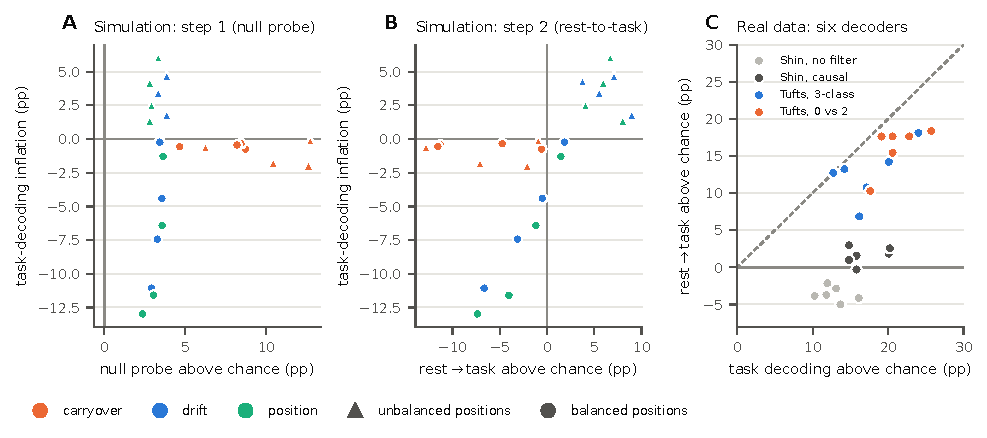
\includegraphics[width=\textwidth]{fig8_diagnostic.pdf}
\caption{Two-step diagnostic. (A, B) Simulation, shared order: task-decoding inflation (task accuracy with a temporal component minus without) against step 1 (A) and step 2 (B), for three components, four task effect sizes, and evaluation over all blocks (balanced positions) or the final three (unbalanced). (C) Real data: rest-to-task transfer against task decoding for six decoders in four settings; points on the dashed line mean that all task accuracy is obtainable from pre-cue windows.}
\label{fig:diag}
\end{figure}

\begin{table}[htbp]
\centering
\caption{Six decoders: excess over chance (pp) for step 1 / step 2 / task decoding. $^{\dagger}$ one-sided Wilcoxon $p\ge 0.01$; all other non-negative entries $p<0.01$; negative entries not tested.}
\label{tab:bench}
\footnotesize
\resizebox{\textwidth}{!}{%
\begin{tabular}{@{}lcccc@{}}
\toprule
Model & Shin, no filter & Shin, causal & Tufts 3-class & Tufts 0 vs 2 \\
\midrule
LogReg & 9.5 / $-3.7$ / 11.8 & 7.4 / 1.0$^{\dagger}$ / 14.8 & 21.1 / 6.9$^{\dagger}$ / 16.2 & 25.7 / 15.4 / 20.6 \\
SVM-RBF & 11.4 / $-4.1$ / 16.1 & 10.8 / 2.6$^{\dagger}$ / 20.2 & 20.6 / 14.2 / 20.1 & 28.7 / 17.6 / 20.6 \\
Random forest & 11.4 / $-2.8$ / 13.1 & 9.1 / 1.9$^{\dagger}$ / 20.1 & 21.6 / 18.1 / 24.0 & 22.1 / 18.4 / 25.7 \\
EEGNet & 9.4 / $-5.0$ / 13.7 & 6.7 / 1.6$^{\dagger}$ / 15.8 & 21.6 / 10.8 / 17.2 & 23.5 / 10.3$^{\dagger}$ / 17.6 \\
DeepConvNet-lite & 5.0 / $-2.1$ / 12.0 & 3.8$^{\dagger}$ / $-0.3$ / 15.8 & 24.0 / 12.7 / 12.7 & 26.5 / 17.6 / 19.1 \\
LSTM & 6.0 / $-3.8$ / 10.3 & 7.3 / 3.0$^{\dagger}$ / 14.8 & 16.7 / 13.2 / 14.2 & 24.3 / 17.6 / 22.8 \\
\midrule
\Rr/task (median) & 0\% & 10\% & 73\% & 76\% \\
\bottomrule
\end{tabular}}
\end{table}

\subsection{Controls}
The drift-injection control stayed at chance with no injected drift (33.8\%), detected half the observed drift (40.1\%) and reproduced the real-data accuracy with the full drift (48.7\% vs 48.0\%; Fig.~\ref{fig:controls}A). WG with per-subject order was at chance (Fig.~\ref{fig:controls}B); its randomisation rule alone, without data, would predict the current label with 62--67\% accuracy, so shared randomisation rules are a weak shared channel in themselves.

\begin{figure}[htbp]
\centering
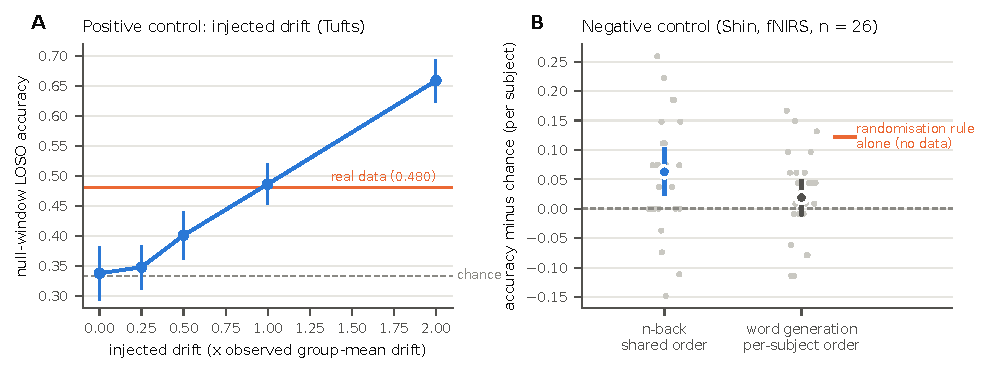
\includegraphics[width=\textwidth]{fig3_controls.pdf}
\caption{Controls. (A) Drift injection in Tufts (mean $\pm$ SD over 20 repetitions). (B) Same participants and causal pipeline: n-back (shared order) versus WG (per-subject order), accuracy minus chance; the orange tick is what the WG randomisation rule alone predicts.}
\label{fig:controls}
\end{figure}

\subsection{Reversed block pairs (Chen Stroop)}
Without any pre-onset window, condition decoding from task windows was above chance for forward pairs (positions 1--2: 65.3\%; 3--4: 57.6\%) and at chance for the reversed pair (47.2\%); forward vs reverse 61.5\% vs 47.2\% (paired $p=0.011$, 15 of 18 participants; supporting; Fig.~\ref{fig:stroop}). Across participants, condition was decodable here only when it agreed with time in session.

\begin{figure}[htbp]
\centering
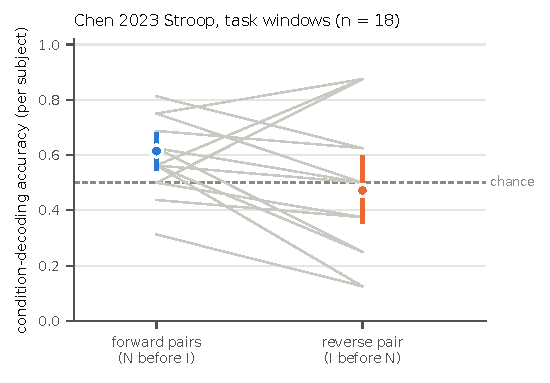
\includegraphics[width=0.55\textwidth]{fig5_stroop.pdf}
\caption{Chen Stroop: condition decoding on forward pairs (neutral first) and on the reverse pair (incongruent first). Lines connect participants.}
\label{fig:stroop}
\end{figure}

\subsection{Published methods}
\textbf{BenchNIRS} reproduced (LDA 39.2\% vs 38.9\% published). With markers shifted 12\,s earlier the same pipeline gave 37.9\% (LOSO; permutation $p=0.008$; published window $p=0.006$), not different from the published window (paired $p=0.74$; Fig.~\ref{fig:repro}A). BenchNIRS epochs include a baseline period and use a zero-phase filter, so its feature window is not cue-free in the sense of Section~\ref{sec:diagnostic}; this result therefore shows that its margin is available before the block, not why.
\textbf{Tufts DeepConvNet} (62.0\% over 16 blocks; 66.5\% on blocks 9--16): its output shifted with session position by 84\% of the 2- vs 0-back effect (Fig.~\ref{fig:benchmark}), without a preceding-block effect ($p=0.71$). Because the Latin square equalises mean position across classes over 16 blocks, this did not raise mean accuracy, exactly as in the balanced-position simulation; it produced position-dependent errors instead.
\textbf{Con4m} reproduced (F1 71.1\% vs 71.28\%) and was unaffected by per-participant block order (69.1--70.6\% in all training/test combinations; Fig.~\ref{fig:repro}B). It uses the task-only release, which contains no rest periods.

\begin{figure}[htbp]
\centering
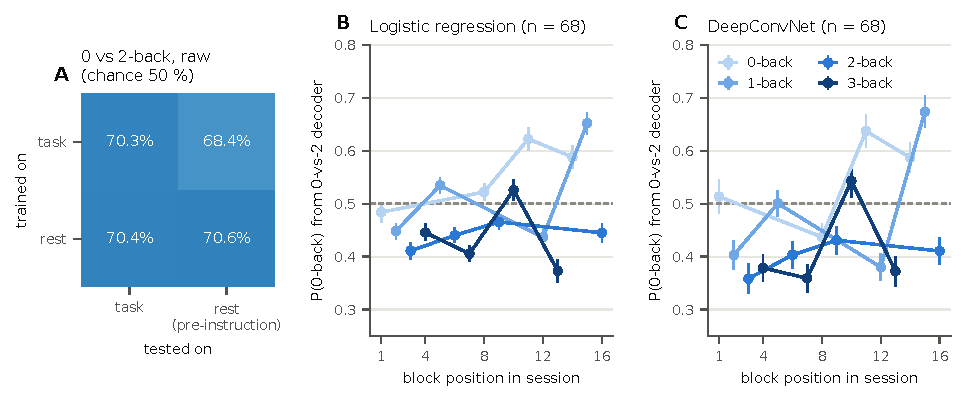
\includegraphics[width=\textwidth]{fig4_benchmark.pdf}
\caption{Tufts official data. (A) Transfer between task and rest-end windows, raw final blocks, 0 vs 2. (B, C) Probability of ``0-back'' from a 0-vs-2 decoder applied to all 16 blocks of held-out participants, by position and true load (mean $\pm$ SEM, $n=68$): (B) logistic regression, (C) official DeepConvNet.}
\label{fig:benchmark}
\end{figure}

\begin{figure}[htbp]
\centering
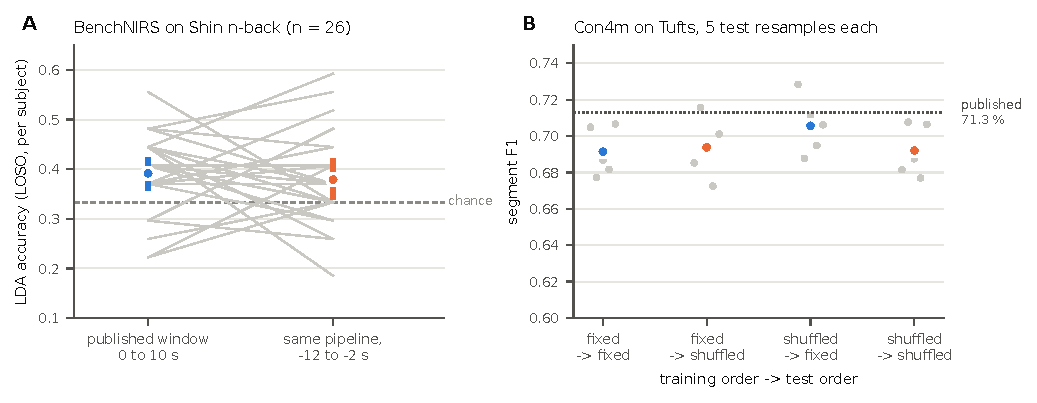
\includegraphics[width=\textwidth]{fig6_reproductions.pdf}
\caption{Re-running published methods. (A) BenchNIRS on Shin: published window versus the same pipeline moved before onset (LOSO, per participant). (B) Con4m on Tufts: segment F1 for every combination of training and test block order; the dotted line is the published F1.}
\label{fig:repro}
\end{figure}

%% ============================================================================
\section{Discussion}
\label{sec:discussion}

Holding out a participant does not hold out a shared sequence. Three findings go beyond earlier work on temporal confounds. First, at the design level, the label information in a sequence and the identifiability of its temporal sources can be computed before any data are analysed; a common remedy, rotating Latin-square rows across participants, removes position information but leaves all first-order transition information. Second, the presence of order information (step 1) and its effect on task decoding (step 2) are different questions with different answers: in Shin the leak is real but arises from carry-over that does not reach the task window, while in Tufts' final blocks most task-decoding accuracy is obtainable without task data. Third, these outcomes were consistent across six decoders within each dataset, and the simulation, in which the truth is known, reproduces both patterns from their mechanisms.

\textbf{Why LOSO restored chance in earlier studies.} Leakage across subjects requires temporal structure that is time-locked to the session and consistent across people. Haemodynamic carry-over, load-dependent rest and shared drift in fNIRS provide it; rapid image presentation in EEG \citep{li2021,ahmed2022} and inert objects \citep{xu2026} do not. Consistent with this, EEG band power in the same windows carried no order information.

\textbf{Apparent inconsistencies are predictable.} The original version of this work reported that some published decoders were affected and others not. The diagnostic explains this: Con4m consumes data without rest periods; DeepConvNet over all 16 Tufts blocks is evaluated with positions balanced across classes, so position effects add errors rather than accuracy; and BenchNIRS uses windows in which the margin is available before the block. A single number such as ``inflation'' is therefore not a property of a model, and we recommend reporting the two diagnostic steps rather than a correction factor.

\textbf{Limitations.} Real-data effects in the most conservative settings are moderate (+5 to +9\pp). Tufts' raw release restricts the probe to three blocks per participant, in which sources are not identifiable; the Tufts decomposition therefore rests on simulation and on the step-2 result. The permutation test was close to but not exactly nominal in simulation, so we required $p<0.01$; Wilcoxon tests for deep networks share this caveat. The simulation's components and magnitudes are a model, not a fit to every dataset. Con4m was run on one split with one seed, and the DeepConvNet re-run used a reduced grid.

\textbf{Recommendations.} (1) Randomise condition order per participant, or use sequences balanced for first-order carry-over \citep{williams1949}; do not rely on Latin squares rotated across subjects. (2) Avoid randomisation rules shared by all participants, or report the accuracy they permit. (3) Release per-participant event timing including rest and cue periods, and check descriptors against the data. (4) For LOSO results on shared-order data, report the null-window probe and rest-to-task transfer, with permutation statistics that re-run the whole pipeline. (5) Avoid zero-phase filters and per-block baselines that overlap the windows compared.

\section{Conclusions}
Shared presentation order is common in public EEG/fNIRS datasets and is not neutralised by subject-independent evaluation. Whether it matters for a reported decoding result is not a property of the model but of the design, the preprocessing and the windows analysed, and it can be assessed with a two-step diagnostic that has been validated against ground truth.

\section*{CRediT authorship contribution statement}
\textbf{Pinzhen He:} Conceptualization, Methodology, Software, Validation, Formal analysis, Investigation, Data curation, Visualization, Writing -- original draft, Writing -- review \& editing.

\section*{Declaration of generative AI and AI-assisted technologies in the writing process}
During the preparation of this work the author used Claude (Anthropic) to assist with literature searching, analysis code, figure generation and drafting of the manuscript text. After using this tool, the author reviewed and edited the content as needed and takes full responsibility for the content of the publication.

\section*{Funding}
This research did not receive any specific grant from funding agencies in the public, commercial, or not-for-profit sectors.

\section*{Declaration of competing interest}
The author declares no competing interests.

\section*{Data availability}
All datasets are public \citep{shin2018,huang2021,chen2023,mukli2021}. Analysis code: \url{https://github.com/huixun160/shared-order-audit}.

\bibliographystyle{elsarticle-num}
\bibliography{refs}

\end{document}
